% Created by tikzDevice version 0.10.1 on 2017-10-05 07:07:40
% !TEX encoding = UTF-8 Unicode
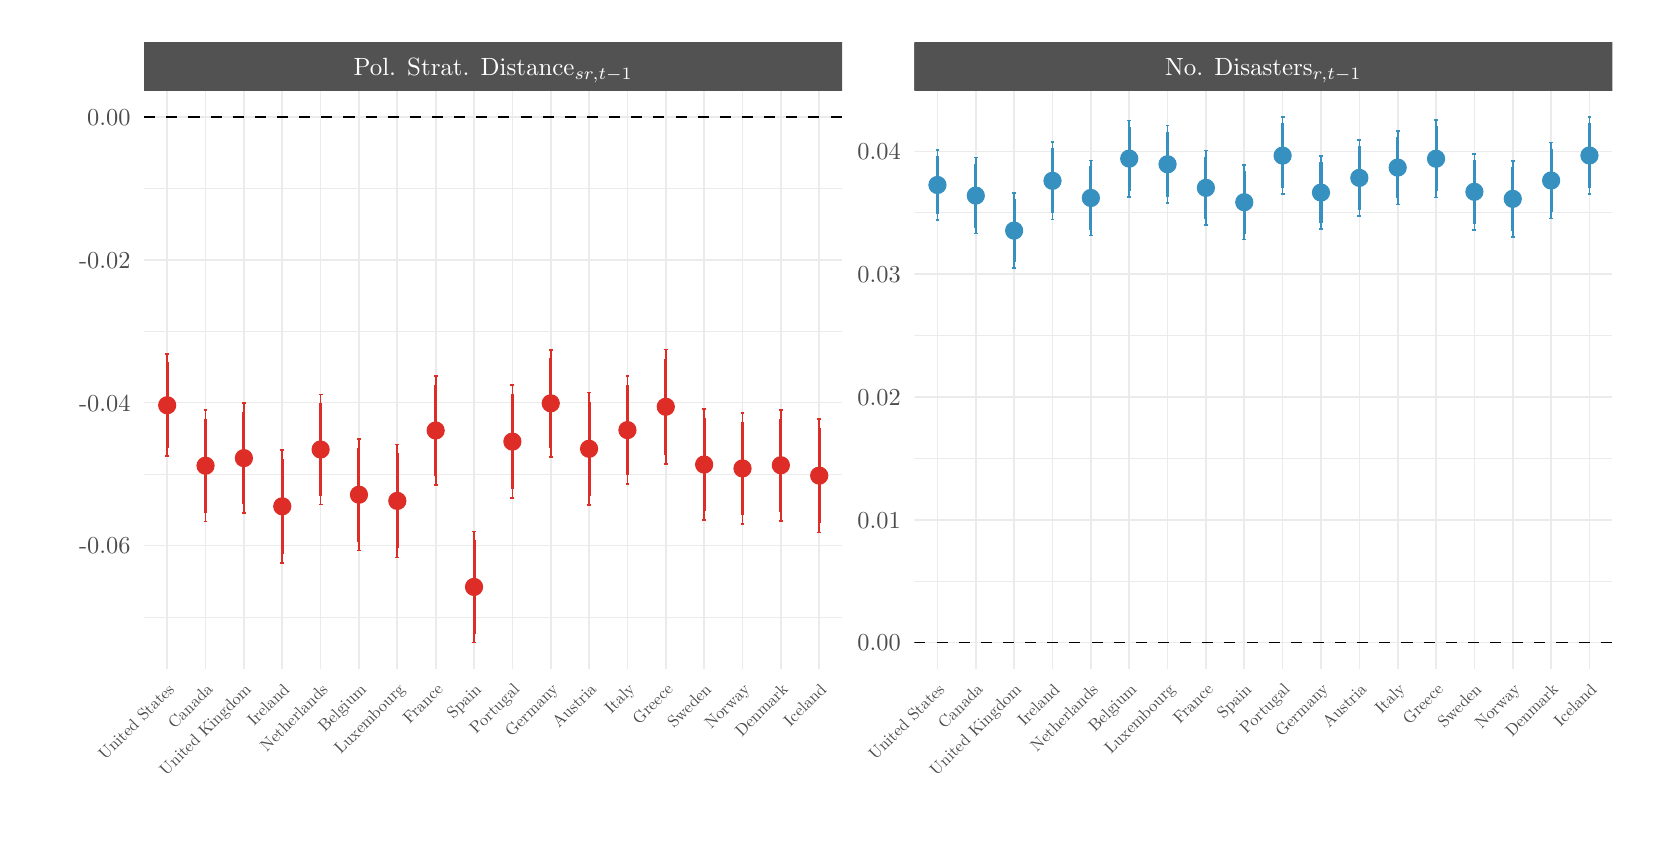
\begin{tikzpicture}[x=1pt,y=1pt]
\definecolor{fillColor}{RGB}{255,255,255}
\path[use as bounding box,fill=fillColor,fill opacity=0.00] (0,0) rectangle (578.16,289.08);
\begin{scope}
\path[clip] (  0.00,  0.00) rectangle (578.16,289.08);
\definecolor{drawColor}{RGB}{255,255,255}
\definecolor{fillColor}{RGB}{255,255,255}

\path[draw=drawColor,line width= 0.6pt,line join=round,line cap=round,fill=fillColor] (  0.00,  0.00) rectangle (578.16,289.08);
\end{scope}
\begin{scope}
\path[clip] ( 42.10, 57.44) rectangle (294.33,266.38);
\definecolor{fillColor}{RGB}{255,255,255}

\path[fill=fillColor] ( 42.10, 57.44) rectangle (294.33,266.38);
\definecolor{drawColor}{gray}{0.92}

\path[draw=drawColor,line width= 0.3pt,line join=round] ( 42.10, 76.10) --
	(294.33, 76.10);

\path[draw=drawColor,line width= 0.3pt,line join=round] ( 42.10,127.75) --
	(294.33,127.75);

\path[draw=drawColor,line width= 0.3pt,line join=round] ( 42.10,179.41) --
	(294.33,179.41);

\path[draw=drawColor,line width= 0.3pt,line join=round] ( 42.10,231.06) --
	(294.33,231.06);

\path[draw=drawColor,line width= 0.6pt,line join=round] ( 42.10,101.93) --
	(294.33,101.93);

\path[draw=drawColor,line width= 0.6pt,line join=round] ( 42.10,153.58) --
	(294.33,153.58);

\path[draw=drawColor,line width= 0.6pt,line join=round] ( 42.10,205.23) --
	(294.33,205.23);

\path[draw=drawColor,line width= 0.6pt,line join=round] ( 42.10,256.88) --
	(294.33,256.88);

\path[draw=drawColor,line width= 0.6pt,line join=round] ( 50.41, 57.44) --
	( 50.41,266.38);

\path[draw=drawColor,line width= 0.6pt,line join=round] ( 64.27, 57.44) --
	( 64.27,266.38);

\path[draw=drawColor,line width= 0.6pt,line join=round] ( 78.13, 57.44) --
	( 78.13,266.38);

\path[draw=drawColor,line width= 0.6pt,line join=round] ( 91.99, 57.44) --
	( 91.99,266.38);

\path[draw=drawColor,line width= 0.6pt,line join=round] (105.85, 57.44) --
	(105.85,266.38);

\path[draw=drawColor,line width= 0.6pt,line join=round] (119.71, 57.44) --
	(119.71,266.38);

\path[draw=drawColor,line width= 0.6pt,line join=round] (133.57, 57.44) --
	(133.57,266.38);

\path[draw=drawColor,line width= 0.6pt,line join=round] (147.43, 57.44) --
	(147.43,266.38);

\path[draw=drawColor,line width= 0.6pt,line join=round] (161.29, 57.44) --
	(161.29,266.38);

\path[draw=drawColor,line width= 0.6pt,line join=round] (175.15, 57.44) --
	(175.15,266.38);

\path[draw=drawColor,line width= 0.6pt,line join=round] (189.01, 57.44) --
	(189.01,266.38);

\path[draw=drawColor,line width= 0.6pt,line join=round] (202.86, 57.44) --
	(202.86,266.38);

\path[draw=drawColor,line width= 0.6pt,line join=round] (216.72, 57.44) --
	(216.72,266.38);

\path[draw=drawColor,line width= 0.6pt,line join=round] (230.58, 57.44) --
	(230.58,266.38);

\path[draw=drawColor,line width= 0.6pt,line join=round] (244.44, 57.44) --
	(244.44,266.38);

\path[draw=drawColor,line width= 0.6pt,line join=round] (258.30, 57.44) --
	(258.30,266.38);

\path[draw=drawColor,line width= 0.6pt,line join=round] (272.16, 57.44) --
	(272.16,266.38);

\path[draw=drawColor,line width= 0.6pt,line join=round] (286.02, 57.44) --
	(286.02,266.38);
\definecolor{drawColor}{RGB}{222,45,38}

\path[draw=drawColor,draw opacity=0.30,line width= 0.3pt,line join=round] ( 50.41,134.22) -- ( 50.41,171.07);

\path[draw=drawColor,draw opacity=0.30,line width= 0.3pt,line join=round] ( 64.27,110.59) -- ( 64.27,150.98);

\path[draw=drawColor,draw opacity=0.30,line width= 0.3pt,line join=round] ( 78.13,113.72) -- ( 78.13,153.36);

\path[draw=drawColor,draw opacity=0.30,line width= 0.3pt,line join=round] ( 91.99, 95.66) -- ( 91.99,136.58);

\path[draw=drawColor,draw opacity=0.30,line width= 0.3pt,line join=round] (105.85,116.78) -- (105.85,156.52);

\path[draw=drawColor,draw opacity=0.30,line width= 0.3pt,line join=round] (119.71,100.11) -- (119.71,140.51);

\path[draw=drawColor,draw opacity=0.30,line width= 0.3pt,line join=round] (133.57, 97.65) -- (133.57,138.51);

\path[draw=drawColor,draw opacity=0.30,line width= 0.3pt,line join=round] (147.43,123.78) -- (147.43,163.25);

\path[draw=drawColor,draw opacity=0.30,line width= 0.3pt,line join=round] (161.29, 66.93) -- (161.29,107.05);

\path[draw=drawColor,draw opacity=0.30,line width= 0.3pt,line join=round] (175.15,119.08) -- (175.15,159.93);

\path[draw=drawColor,draw opacity=0.30,line width= 0.3pt,line join=round] (189.01,133.97) -- (189.01,172.71);

\path[draw=drawColor,draw opacity=0.30,line width= 0.3pt,line join=round] (202.86,116.59) -- (202.86,157.24);

\path[draw=drawColor,draw opacity=0.30,line width= 0.3pt,line join=round] (216.72,124.23) -- (216.72,163.11);

\path[draw=drawColor,draw opacity=0.30,line width= 0.3pt,line join=round] (230.58,131.42) -- (230.58,172.76);

\path[draw=drawColor,draw opacity=0.30,line width= 0.3pt,line join=round] (244.44,111.13) -- (244.44,151.28);

\path[draw=drawColor,draw opacity=0.30,line width= 0.3pt,line join=round] (258.30,109.69) -- (258.30,149.94);

\path[draw=drawColor,draw opacity=0.30,line width= 0.3pt,line join=round] (272.16,110.90) -- (272.16,151.03);

\path[draw=drawColor,draw opacity=0.30,line width= 0.3pt,line join=round] (286.02,106.65) -- (286.02,147.77);
\definecolor{drawColor}{RGB}{222,45,38}

\path[draw=drawColor,line width= 1.1pt,line join=round] ( 50.41,137.18) -- ( 50.41,168.10);

\path[draw=drawColor,line width= 1.1pt,line join=round] ( 64.27,113.84) -- ( 64.27,147.74);

\path[draw=drawColor,line width= 1.1pt,line join=round] ( 78.13,116.91) -- ( 78.13,150.18);

\path[draw=drawColor,line width= 1.1pt,line join=round] ( 91.99, 98.95) -- ( 91.99,133.29);

\path[draw=drawColor,line width= 1.1pt,line join=round] (105.85,119.98) -- (105.85,153.32);

\path[draw=drawColor,line width= 1.1pt,line join=round] (119.71,103.36) -- (119.71,137.27);

\path[draw=drawColor,line width= 1.1pt,line join=round] (133.57,100.93) -- (133.57,135.22);

\path[draw=drawColor,line width= 1.1pt,line join=round] (147.43,126.95) -- (147.43,160.08);

\path[draw=drawColor,line width= 1.1pt,line join=round] (161.29, 70.16) -- (161.29,103.82);

\path[draw=drawColor,line width= 1.1pt,line join=round] (175.15,122.36) -- (175.15,156.65);

\path[draw=drawColor,line width= 1.1pt,line join=round] (189.01,137.09) -- (189.01,169.59);

\path[draw=drawColor,line width= 1.1pt,line join=round] (202.86,119.86) -- (202.86,153.97);

\path[draw=drawColor,line width= 1.1pt,line join=round] (216.72,127.36) -- (216.72,159.99);

\path[draw=drawColor,line width= 1.1pt,line join=round] (230.58,134.74) -- (230.58,169.43);

\path[draw=drawColor,line width= 1.1pt,line join=round] (244.44,114.36) -- (244.44,148.05);

\path[draw=drawColor,line width= 1.1pt,line join=round] (258.30,112.92) -- (258.30,146.70);

\path[draw=drawColor,line width= 1.1pt,line join=round] (272.16,114.12) -- (272.16,147.80);

\path[draw=drawColor,line width= 1.1pt,line join=round] (286.02,109.96) -- (286.02,144.47);
\definecolor{drawColor}{RGB}{0,0,0}

\path[draw=drawColor,line width= 0.6pt,dash pattern=on 4pt off 4pt ,line join=round] ( 42.10,256.88) -- (294.33,256.88);
\definecolor{drawColor}{RGB}{222,45,38}
\definecolor{fillColor}{RGB}{222,45,38}

\path[draw=drawColor,line width= 0.4pt,line join=round,line cap=round,fill=fillColor] ( 50.41,152.64) circle (  3.09);

\path[draw=drawColor,line width= 0.4pt,line join=round,line cap=round,fill=fillColor] ( 64.27,130.79) circle (  3.09);

\path[draw=drawColor,line width= 0.4pt,line join=round,line cap=round,fill=fillColor] ( 78.13,133.54) circle (  3.09);

\path[draw=drawColor,line width= 0.4pt,line join=round,line cap=round,fill=fillColor] ( 91.99,116.12) circle (  3.09);

\path[draw=drawColor,line width= 0.4pt,line join=round,line cap=round,fill=fillColor] (105.85,136.65) circle (  3.09);

\path[draw=drawColor,line width= 0.4pt,line join=round,line cap=round,fill=fillColor] (119.71,120.31) circle (  3.09);

\path[draw=drawColor,line width= 0.4pt,line join=round,line cap=round,fill=fillColor] (133.57,118.08) circle (  3.09);

\path[draw=drawColor,line width= 0.4pt,line join=round,line cap=round,fill=fillColor] (147.43,143.52) circle (  3.09);

\path[draw=drawColor,line width= 0.4pt,line join=round,line cap=round,fill=fillColor] (161.29, 86.99) circle (  3.09);

\path[draw=drawColor,line width= 0.4pt,line join=round,line cap=round,fill=fillColor] (175.15,139.51) circle (  3.09);

\path[draw=drawColor,line width= 0.4pt,line join=round,line cap=round,fill=fillColor] (189.01,153.34) circle (  3.09);

\path[draw=drawColor,line width= 0.4pt,line join=round,line cap=round,fill=fillColor] (202.86,136.91) circle (  3.09);

\path[draw=drawColor,line width= 0.4pt,line join=round,line cap=round,fill=fillColor] (216.72,143.67) circle (  3.09);

\path[draw=drawColor,line width= 0.4pt,line join=round,line cap=round,fill=fillColor] (230.58,152.09) circle (  3.09);

\path[draw=drawColor,line width= 0.4pt,line join=round,line cap=round,fill=fillColor] (244.44,131.21) circle (  3.09);

\path[draw=drawColor,line width= 0.4pt,line join=round,line cap=round,fill=fillColor] (258.30,129.81) circle (  3.09);

\path[draw=drawColor,line width= 0.4pt,line join=round,line cap=round,fill=fillColor] (272.16,130.96) circle (  3.09);

\path[draw=drawColor,line width= 0.4pt,line join=round,line cap=round,fill=fillColor] (286.02,127.21) circle (  3.09);

\path[draw=drawColor,line width= 0.6pt,line join=round] ( 49.72,171.07) --
	( 51.11,171.07);

\path[draw=drawColor,line width= 0.6pt,line join=round] ( 50.41,171.07) --
	( 50.41,134.22);

\path[draw=drawColor,line width= 0.6pt,line join=round] ( 49.72,134.22) --
	( 51.11,134.22);

\path[draw=drawColor,line width= 0.6pt,line join=round] ( 63.58,150.98) --
	( 64.97,150.98);

\path[draw=drawColor,line width= 0.6pt,line join=round] ( 64.27,150.98) --
	( 64.27,110.59);

\path[draw=drawColor,line width= 0.6pt,line join=round] ( 63.58,110.59) --
	( 64.97,110.59);

\path[draw=drawColor,line width= 0.6pt,line join=round] ( 77.44,153.36) --
	( 78.83,153.36);

\path[draw=drawColor,line width= 0.6pt,line join=round] ( 78.13,153.36) --
	( 78.13,113.72);

\path[draw=drawColor,line width= 0.6pt,line join=round] ( 77.44,113.72) --
	( 78.83,113.72);

\path[draw=drawColor,line width= 0.6pt,line join=round] ( 91.30,136.58) --
	( 92.68,136.58);

\path[draw=drawColor,line width= 0.6pt,line join=round] ( 91.99,136.58) --
	( 91.99, 95.66);

\path[draw=drawColor,line width= 0.6pt,line join=round] ( 91.30, 95.66) --
	( 92.68, 95.66);

\path[draw=drawColor,line width= 0.6pt,line join=round] (105.16,156.52) --
	(106.54,156.52);

\path[draw=drawColor,line width= 0.6pt,line join=round] (105.85,156.52) --
	(105.85,116.78);

\path[draw=drawColor,line width= 0.6pt,line join=round] (105.16,116.78) --
	(106.54,116.78);

\path[draw=drawColor,line width= 0.6pt,line join=round] (119.02,140.51) --
	(120.40,140.51);

\path[draw=drawColor,line width= 0.6pt,line join=round] (119.71,140.51) --
	(119.71,100.11);

\path[draw=drawColor,line width= 0.6pt,line join=round] (119.02,100.11) --
	(120.40,100.11);

\path[draw=drawColor,line width= 0.6pt,line join=round] (132.88,138.51) --
	(134.26,138.51);

\path[draw=drawColor,line width= 0.6pt,line join=round] (133.57,138.51) --
	(133.57, 97.65);

\path[draw=drawColor,line width= 0.6pt,line join=round] (132.88, 97.65) --
	(134.26, 97.65);

\path[draw=drawColor,line width= 0.6pt,line join=round] (146.74,163.25) --
	(148.12,163.25);

\path[draw=drawColor,line width= 0.6pt,line join=round] (147.43,163.25) --
	(147.43,123.78);

\path[draw=drawColor,line width= 0.6pt,line join=round] (146.74,123.78) --
	(148.12,123.78);

\path[draw=drawColor,line width= 0.6pt,line join=round] (160.59,107.05) --
	(161.98,107.05);

\path[draw=drawColor,line width= 0.6pt,line join=round] (161.29,107.05) --
	(161.29, 66.93);

\path[draw=drawColor,line width= 0.6pt,line join=round] (160.59, 66.93) --
	(161.98, 66.93);

\path[draw=drawColor,line width= 0.6pt,line join=round] (174.45,159.93) --
	(175.84,159.93);

\path[draw=drawColor,line width= 0.6pt,line join=round] (175.15,159.93) --
	(175.15,119.08);

\path[draw=drawColor,line width= 0.6pt,line join=round] (174.45,119.08) --
	(175.84,119.08);

\path[draw=drawColor,line width= 0.6pt,line join=round] (188.31,172.71) --
	(189.70,172.71);

\path[draw=drawColor,line width= 0.6pt,line join=round] (189.01,172.71) --
	(189.01,133.97);

\path[draw=drawColor,line width= 0.6pt,line join=round] (188.31,133.97) --
	(189.70,133.97);

\path[draw=drawColor,line width= 0.6pt,line join=round] (202.17,157.24) --
	(203.56,157.24);

\path[draw=drawColor,line width= 0.6pt,line join=round] (202.86,157.24) --
	(202.86,116.59);

\path[draw=drawColor,line width= 0.6pt,line join=round] (202.17,116.59) --
	(203.56,116.59);

\path[draw=drawColor,line width= 0.6pt,line join=round] (216.03,163.11) --
	(217.42,163.11);

\path[draw=drawColor,line width= 0.6pt,line join=round] (216.72,163.11) --
	(216.72,124.23);

\path[draw=drawColor,line width= 0.6pt,line join=round] (216.03,124.23) --
	(217.42,124.23);

\path[draw=drawColor,line width= 0.6pt,line join=round] (229.89,172.76) --
	(231.28,172.76);

\path[draw=drawColor,line width= 0.6pt,line join=round] (230.58,172.76) --
	(230.58,131.42);

\path[draw=drawColor,line width= 0.6pt,line join=round] (229.89,131.42) --
	(231.28,131.42);

\path[draw=drawColor,line width= 0.6pt,line join=round] (243.75,151.28) --
	(245.13,151.28);

\path[draw=drawColor,line width= 0.6pt,line join=round] (244.44,151.28) --
	(244.44,111.13);

\path[draw=drawColor,line width= 0.6pt,line join=round] (243.75,111.13) --
	(245.13,111.13);

\path[draw=drawColor,line width= 0.6pt,line join=round] (257.61,149.94) --
	(258.99,149.94);

\path[draw=drawColor,line width= 0.6pt,line join=round] (258.30,149.94) --
	(258.30,109.69);

\path[draw=drawColor,line width= 0.6pt,line join=round] (257.61,109.69) --
	(258.99,109.69);

\path[draw=drawColor,line width= 0.6pt,line join=round] (271.47,151.03) --
	(272.85,151.03);

\path[draw=drawColor,line width= 0.6pt,line join=round] (272.16,151.03) --
	(272.16,110.90);

\path[draw=drawColor,line width= 0.6pt,line join=round] (271.47,110.90) --
	(272.85,110.90);

\path[draw=drawColor,line width= 0.6pt,line join=round] (285.33,147.77) --
	(286.71,147.77);

\path[draw=drawColor,line width= 0.6pt,line join=round] (286.02,147.77) --
	(286.02,106.65);

\path[draw=drawColor,line width= 0.6pt,line join=round] (285.33,106.65) --
	(286.71,106.65);
\end{scope}
\begin{scope}
\path[clip] (320.42, 57.44) rectangle (572.66,266.38);
\definecolor{fillColor}{RGB}{255,255,255}

\path[fill=fillColor] (320.42, 57.44) rectangle (572.66,266.38);
\definecolor{drawColor}{gray}{0.92}

\path[draw=drawColor,line width= 0.3pt,line join=round] (320.42, 89.11) --
	(572.66, 89.11);

\path[draw=drawColor,line width= 0.3pt,line join=round] (320.42,133.47) --
	(572.66,133.47);

\path[draw=drawColor,line width= 0.3pt,line join=round] (320.42,177.82) --
	(572.66,177.82);

\path[draw=drawColor,line width= 0.3pt,line join=round] (320.42,222.18) --
	(572.66,222.18);

\path[draw=drawColor,line width= 0.6pt,line join=round] (320.42, 66.93) --
	(572.66, 66.93);

\path[draw=drawColor,line width= 0.6pt,line join=round] (320.42,111.29) --
	(572.66,111.29);

\path[draw=drawColor,line width= 0.6pt,line join=round] (320.42,155.64) --
	(572.66,155.64);

\path[draw=drawColor,line width= 0.6pt,line join=round] (320.42,200.00) --
	(572.66,200.00);

\path[draw=drawColor,line width= 0.6pt,line join=round] (320.42,244.35) --
	(572.66,244.35);

\path[draw=drawColor,line width= 0.6pt,line join=round] (328.74, 57.44) --
	(328.74,266.38);

\path[draw=drawColor,line width= 0.6pt,line join=round] (342.60, 57.44) --
	(342.60,266.38);

\path[draw=drawColor,line width= 0.6pt,line join=round] (356.46, 57.44) --
	(356.46,266.38);

\path[draw=drawColor,line width= 0.6pt,line join=round] (370.32, 57.44) --
	(370.32,266.38);

\path[draw=drawColor,line width= 0.6pt,line join=round] (384.18, 57.44) --
	(384.18,266.38);

\path[draw=drawColor,line width= 0.6pt,line join=round] (398.04, 57.44) --
	(398.04,266.38);

\path[draw=drawColor,line width= 0.6pt,line join=round] (411.89, 57.44) --
	(411.89,266.38);

\path[draw=drawColor,line width= 0.6pt,line join=round] (425.75, 57.44) --
	(425.75,266.38);

\path[draw=drawColor,line width= 0.6pt,line join=round] (439.61, 57.44) --
	(439.61,266.38);

\path[draw=drawColor,line width= 0.6pt,line join=round] (453.47, 57.44) --
	(453.47,266.38);

\path[draw=drawColor,line width= 0.6pt,line join=round] (467.33, 57.44) --
	(467.33,266.38);

\path[draw=drawColor,line width= 0.6pt,line join=round] (481.19, 57.44) --
	(481.19,266.38);

\path[draw=drawColor,line width= 0.6pt,line join=round] (495.05, 57.44) --
	(495.05,266.38);

\path[draw=drawColor,line width= 0.6pt,line join=round] (508.91, 57.44) --
	(508.91,266.38);

\path[draw=drawColor,line width= 0.6pt,line join=round] (522.77, 57.44) --
	(522.77,266.38);

\path[draw=drawColor,line width= 0.6pt,line join=round] (536.63, 57.44) --
	(536.63,266.38);

\path[draw=drawColor,line width= 0.6pt,line join=round] (550.49, 57.44) --
	(550.49,266.38);

\path[draw=drawColor,line width= 0.6pt,line join=round] (564.34, 57.44) --
	(564.34,266.38);
\definecolor{drawColor}{RGB}{54,144,192}

\path[draw=drawColor,draw opacity=0.30,line width= 0.3pt,line join=round] (328.74,219.59) -- (328.74,244.87);

\path[draw=drawColor,draw opacity=0.30,line width= 0.3pt,line join=round] (342.60,214.65) -- (342.60,242.12);

\path[draw=drawColor,draw opacity=0.30,line width= 0.3pt,line join=round] (356.46,202.18) -- (356.46,229.30);

\path[draw=drawColor,draw opacity=0.30,line width= 0.3pt,line join=round] (370.32,219.80) -- (370.32,247.68);

\path[draw=drawColor,draw opacity=0.30,line width= 0.3pt,line join=round] (384.18,213.94) -- (384.18,241.13);

\path[draw=drawColor,draw opacity=0.30,line width= 0.3pt,line join=round] (398.04,227.94) -- (398.04,255.57);

\path[draw=drawColor,draw opacity=0.30,line width= 0.3pt,line join=round] (411.89,225.75) -- (411.89,253.67);

\path[draw=drawColor,draw opacity=0.30,line width= 0.3pt,line join=round] (425.75,217.70) -- (425.75,244.69);

\path[draw=drawColor,draw opacity=0.30,line width= 0.3pt,line join=round] (439.61,212.48) -- (439.61,239.53);

\path[draw=drawColor,draw opacity=0.30,line width= 0.3pt,line join=round] (453.47,228.94) -- (453.47,256.76);

\path[draw=drawColor,draw opacity=0.30,line width= 0.3pt,line join=round] (467.33,216.23) -- (467.33,242.76);

\path[draw=drawColor,draw opacity=0.30,line width= 0.3pt,line join=round] (481.19,221.01) -- (481.19,248.59);

\path[draw=drawColor,draw opacity=0.30,line width= 0.3pt,line join=round] (495.05,225.21) -- (495.05,251.82);

\path[draw=drawColor,draw opacity=0.30,line width= 0.3pt,line join=round] (508.91,227.76) -- (508.91,255.69);

\path[draw=drawColor,draw opacity=0.30,line width= 0.3pt,line join=round] (522.77,216.08) -- (522.77,243.47);

\path[draw=drawColor,draw opacity=0.30,line width= 0.3pt,line join=round] (536.63,213.49) -- (536.63,240.95);

\path[draw=drawColor,draw opacity=0.30,line width= 0.3pt,line join=round] (550.49,220.13) -- (550.49,247.57);

\path[draw=drawColor,draw opacity=0.30,line width= 0.3pt,line join=round] (564.34,228.90) -- (564.34,256.88);
\definecolor{drawColor}{RGB}{54,144,192}

\path[draw=drawColor,line width= 1.1pt,line join=round] (328.74,221.62) -- (328.74,242.84);

\path[draw=drawColor,line width= 1.1pt,line join=round] (342.60,216.86) -- (342.60,239.91);

\path[draw=drawColor,line width= 1.1pt,line join=round] (356.46,204.36) -- (356.46,227.12);

\path[draw=drawColor,line width= 1.1pt,line join=round] (370.32,222.04) -- (370.32,245.44);

\path[draw=drawColor,line width= 1.1pt,line join=round] (384.18,216.12) -- (384.18,238.95);

\path[draw=drawColor,line width= 1.1pt,line join=round] (398.04,230.16) -- (398.04,253.35);

\path[draw=drawColor,line width= 1.1pt,line join=round] (411.89,227.99) -- (411.89,251.42);

\path[draw=drawColor,line width= 1.1pt,line join=round] (425.75,219.87) -- (425.75,242.52);

\path[draw=drawColor,line width= 1.1pt,line join=round] (439.61,214.65) -- (439.61,237.36);

\path[draw=drawColor,line width= 1.1pt,line join=round] (453.47,231.17) -- (453.47,254.52);

\path[draw=drawColor,line width= 1.1pt,line join=round] (467.33,218.36) -- (467.33,240.62);

\path[draw=drawColor,line width= 1.1pt,line join=round] (481.19,223.23) -- (481.19,246.38);

\path[draw=drawColor,line width= 1.1pt,line join=round] (495.05,227.35) -- (495.05,249.68);

\path[draw=drawColor,line width= 1.1pt,line join=round] (508.91,230.00) -- (508.91,253.44);

\path[draw=drawColor,line width= 1.1pt,line join=round] (522.77,218.28) -- (522.77,241.27);

\path[draw=drawColor,line width= 1.1pt,line join=round] (536.63,215.70) -- (536.63,238.74);

\path[draw=drawColor,line width= 1.1pt,line join=round] (550.49,222.34) -- (550.49,245.36);

\path[draw=drawColor,line width= 1.1pt,line join=round] (564.34,231.15) -- (564.34,254.63);
\definecolor{drawColor}{RGB}{0,0,0}

\path[draw=drawColor,line width= 0.6pt,dash pattern=on 4pt off 4pt ,line join=round] (320.42, 66.93) -- (572.66, 66.93);
\definecolor{drawColor}{RGB}{54,144,192}
\definecolor{fillColor}{RGB}{54,144,192}

\path[draw=drawColor,line width= 0.4pt,line join=round,line cap=round,fill=fillColor] (328.74,232.23) circle (  3.09);

\path[draw=drawColor,line width= 0.4pt,line join=round,line cap=round,fill=fillColor] (342.60,228.39) circle (  3.09);

\path[draw=drawColor,line width= 0.4pt,line join=round,line cap=round,fill=fillColor] (356.46,215.74) circle (  3.09);

\path[draw=drawColor,line width= 0.4pt,line join=round,line cap=round,fill=fillColor] (370.32,233.74) circle (  3.09);

\path[draw=drawColor,line width= 0.4pt,line join=round,line cap=round,fill=fillColor] (384.18,227.54) circle (  3.09);

\path[draw=drawColor,line width= 0.4pt,line join=round,line cap=round,fill=fillColor] (398.04,241.76) circle (  3.09);

\path[draw=drawColor,line width= 0.4pt,line join=round,line cap=round,fill=fillColor] (411.89,239.71) circle (  3.09);

\path[draw=drawColor,line width= 0.4pt,line join=round,line cap=round,fill=fillColor] (425.75,231.19) circle (  3.09);

\path[draw=drawColor,line width= 0.4pt,line join=round,line cap=round,fill=fillColor] (439.61,226.00) circle (  3.09);

\path[draw=drawColor,line width= 0.4pt,line join=round,line cap=round,fill=fillColor] (453.47,242.85) circle (  3.09);

\path[draw=drawColor,line width= 0.4pt,line join=round,line cap=round,fill=fillColor] (467.33,229.49) circle (  3.09);

\path[draw=drawColor,line width= 0.4pt,line join=round,line cap=round,fill=fillColor] (481.19,234.80) circle (  3.09);

\path[draw=drawColor,line width= 0.4pt,line join=round,line cap=round,fill=fillColor] (495.05,238.52) circle (  3.09);

\path[draw=drawColor,line width= 0.4pt,line join=round,line cap=round,fill=fillColor] (508.91,241.72) circle (  3.09);

\path[draw=drawColor,line width= 0.4pt,line join=round,line cap=round,fill=fillColor] (522.77,229.77) circle (  3.09);

\path[draw=drawColor,line width= 0.4pt,line join=round,line cap=round,fill=fillColor] (536.63,227.22) circle (  3.09);

\path[draw=drawColor,line width= 0.4pt,line join=round,line cap=round,fill=fillColor] (550.49,233.85) circle (  3.09);

\path[draw=drawColor,line width= 0.4pt,line join=round,line cap=round,fill=fillColor] (564.34,242.89) circle (  3.09);

\path[draw=drawColor,line width= 0.6pt,line join=round] (328.05,244.87) --
	(329.43,244.87);

\path[draw=drawColor,line width= 0.6pt,line join=round] (328.74,244.87) --
	(328.74,219.59);

\path[draw=drawColor,line width= 0.6pt,line join=round] (328.05,219.59) --
	(329.43,219.59);

\path[draw=drawColor,line width= 0.6pt,line join=round] (341.91,242.12) --
	(343.29,242.12);

\path[draw=drawColor,line width= 0.6pt,line join=round] (342.60,242.12) --
	(342.60,214.65);

\path[draw=drawColor,line width= 0.6pt,line join=round] (341.91,214.65) --
	(343.29,214.65);

\path[draw=drawColor,line width= 0.6pt,line join=round] (355.77,229.30) --
	(357.15,229.30);

\path[draw=drawColor,line width= 0.6pt,line join=round] (356.46,229.30) --
	(356.46,202.18);

\path[draw=drawColor,line width= 0.6pt,line join=round] (355.77,202.18) --
	(357.15,202.18);

\path[draw=drawColor,line width= 0.6pt,line join=round] (369.62,247.68) --
	(371.01,247.68);

\path[draw=drawColor,line width= 0.6pt,line join=round] (370.32,247.68) --
	(370.32,219.80);

\path[draw=drawColor,line width= 0.6pt,line join=round] (369.62,219.80) --
	(371.01,219.80);

\path[draw=drawColor,line width= 0.6pt,line join=round] (383.48,241.13) --
	(384.87,241.13);

\path[draw=drawColor,line width= 0.6pt,line join=round] (384.18,241.13) --
	(384.18,213.94);

\path[draw=drawColor,line width= 0.6pt,line join=round] (383.48,213.94) --
	(384.87,213.94);

\path[draw=drawColor,line width= 0.6pt,line join=round] (397.34,255.57) --
	(398.73,255.57);

\path[draw=drawColor,line width= 0.6pt,line join=round] (398.04,255.57) --
	(398.04,227.94);

\path[draw=drawColor,line width= 0.6pt,line join=round] (397.34,227.94) --
	(398.73,227.94);

\path[draw=drawColor,line width= 0.6pt,line join=round] (411.20,253.67) --
	(412.59,253.67);

\path[draw=drawColor,line width= 0.6pt,line join=round] (411.89,253.67) --
	(411.89,225.75);

\path[draw=drawColor,line width= 0.6pt,line join=round] (411.20,225.75) --
	(412.59,225.75);

\path[draw=drawColor,line width= 0.6pt,line join=round] (425.06,244.69) --
	(426.45,244.69);

\path[draw=drawColor,line width= 0.6pt,line join=round] (425.75,244.69) --
	(425.75,217.70);

\path[draw=drawColor,line width= 0.6pt,line join=round] (425.06,217.70) --
	(426.45,217.70);

\path[draw=drawColor,line width= 0.6pt,line join=round] (438.92,239.53) --
	(440.31,239.53);

\path[draw=drawColor,line width= 0.6pt,line join=round] (439.61,239.53) --
	(439.61,212.48);

\path[draw=drawColor,line width= 0.6pt,line join=round] (438.92,212.48) --
	(440.31,212.48);

\path[draw=drawColor,line width= 0.6pt,line join=round] (452.78,256.76) --
	(454.16,256.76);

\path[draw=drawColor,line width= 0.6pt,line join=round] (453.47,256.76) --
	(453.47,228.94);

\path[draw=drawColor,line width= 0.6pt,line join=round] (452.78,228.94) --
	(454.16,228.94);

\path[draw=drawColor,line width= 0.6pt,line join=round] (466.64,242.76) --
	(468.02,242.76);

\path[draw=drawColor,line width= 0.6pt,line join=round] (467.33,242.76) --
	(467.33,216.23);

\path[draw=drawColor,line width= 0.6pt,line join=round] (466.64,216.23) --
	(468.02,216.23);

\path[draw=drawColor,line width= 0.6pt,line join=round] (480.50,248.59) --
	(481.88,248.59);

\path[draw=drawColor,line width= 0.6pt,line join=round] (481.19,248.59) --
	(481.19,221.01);

\path[draw=drawColor,line width= 0.6pt,line join=round] (480.50,221.01) --
	(481.88,221.01);

\path[draw=drawColor,line width= 0.6pt,line join=round] (494.36,251.82) --
	(495.74,251.82);

\path[draw=drawColor,line width= 0.6pt,line join=round] (495.05,251.82) --
	(495.05,225.21);

\path[draw=drawColor,line width= 0.6pt,line join=round] (494.36,225.21) --
	(495.74,225.21);

\path[draw=drawColor,line width= 0.6pt,line join=round] (508.22,255.69) --
	(509.60,255.69);

\path[draw=drawColor,line width= 0.6pt,line join=round] (508.91,255.69) --
	(508.91,227.76);

\path[draw=drawColor,line width= 0.6pt,line join=round] (508.22,227.76) --
	(509.60,227.76);

\path[draw=drawColor,line width= 0.6pt,line join=round] (522.07,243.47) --
	(523.46,243.47);

\path[draw=drawColor,line width= 0.6pt,line join=round] (522.77,243.47) --
	(522.77,216.08);

\path[draw=drawColor,line width= 0.6pt,line join=round] (522.07,216.08) --
	(523.46,216.08);

\path[draw=drawColor,line width= 0.6pt,line join=round] (535.93,240.95) --
	(537.32,240.95);

\path[draw=drawColor,line width= 0.6pt,line join=round] (536.63,240.95) --
	(536.63,213.49);

\path[draw=drawColor,line width= 0.6pt,line join=round] (535.93,213.49) --
	(537.32,213.49);

\path[draw=drawColor,line width= 0.6pt,line join=round] (549.79,247.57) --
	(551.18,247.57);

\path[draw=drawColor,line width= 0.6pt,line join=round] (550.49,247.57) --
	(550.49,220.13);

\path[draw=drawColor,line width= 0.6pt,line join=round] (549.79,220.13) --
	(551.18,220.13);

\path[draw=drawColor,line width= 0.6pt,line join=round] (563.65,256.88) --
	(565.04,256.88);

\path[draw=drawColor,line width= 0.6pt,line join=round] (564.34,256.88) --
	(564.34,228.90);

\path[draw=drawColor,line width= 0.6pt,line join=round] (563.65,228.90) --
	(565.04,228.90);
\end{scope}
\begin{scope}
\path[clip] ( 42.10,266.38) rectangle (294.33,283.58);
\definecolor{drawColor}{gray}{0.32}
\definecolor{fillColor}{gray}{0.32}

\path[draw=drawColor,line width= 0.6pt,line join=round,line cap=round,fill=fillColor] ( 42.10,266.38) rectangle (294.33,283.58);
\definecolor{drawColor}{RGB}{255,255,255}

\node[text=drawColor,anchor=base,inner sep=0pt, outer sep=0pt, scale=  0.90] at (168.22,271.88) {Pol. Strat. Distance$_{sr,t-1}$};
\end{scope}
\begin{scope}
\path[clip] (320.42,266.38) rectangle (572.66,283.58);
\definecolor{drawColor}{gray}{0.32}
\definecolor{fillColor}{gray}{0.32}

\path[draw=drawColor,line width= 0.6pt,line join=round,line cap=round,fill=fillColor] (320.42,266.38) rectangle (572.66,283.58);
\definecolor{drawColor}{RGB}{255,255,255}

\node[text=drawColor,anchor=base,inner sep=0pt, outer sep=0pt, scale=  0.90] at (446.54,271.88) {No. Disasters$_{r,t-1}$};
\end{scope}
\begin{scope}
\path[clip] (  0.00,  0.00) rectangle (578.16,289.08);
\definecolor{drawColor}{gray}{0.30}

\node[text=drawColor,rotate= 45.00,anchor=base east,inner sep=0pt, outer sep=0pt, scale=  0.60] at ( 53.34, 49.56) {United States};

\node[text=drawColor,rotate= 45.00,anchor=base east,inner sep=0pt, outer sep=0pt, scale=  0.60] at ( 67.20, 49.56) {Canada};

\node[text=drawColor,rotate= 45.00,anchor=base east,inner sep=0pt, outer sep=0pt, scale=  0.60] at ( 81.05, 49.56) {United Kingdom};

\node[text=drawColor,rotate= 45.00,anchor=base east,inner sep=0pt, outer sep=0pt, scale=  0.60] at ( 94.91, 49.56) {Ireland};

\node[text=drawColor,rotate= 45.00,anchor=base east,inner sep=0pt, outer sep=0pt, scale=  0.60] at (108.77, 49.56) {Netherlands};

\node[text=drawColor,rotate= 45.00,anchor=base east,inner sep=0pt, outer sep=0pt, scale=  0.60] at (122.63, 49.56) {Belgium};

\node[text=drawColor,rotate= 45.00,anchor=base east,inner sep=0pt, outer sep=0pt, scale=  0.60] at (136.49, 49.56) {Luxembourg};

\node[text=drawColor,rotate= 45.00,anchor=base east,inner sep=0pt, outer sep=0pt, scale=  0.60] at (150.35, 49.56) {France};

\node[text=drawColor,rotate= 45.00,anchor=base east,inner sep=0pt, outer sep=0pt, scale=  0.60] at (164.21, 49.56) {Spain};

\node[text=drawColor,rotate= 45.00,anchor=base east,inner sep=0pt, outer sep=0pt, scale=  0.60] at (178.07, 49.56) {Portugal};

\node[text=drawColor,rotate= 45.00,anchor=base east,inner sep=0pt, outer sep=0pt, scale=  0.60] at (191.93, 49.56) {Germany};

\node[text=drawColor,rotate= 45.00,anchor=base east,inner sep=0pt, outer sep=0pt, scale=  0.60] at (205.79, 49.56) {Austria};

\node[text=drawColor,rotate= 45.00,anchor=base east,inner sep=0pt, outer sep=0pt, scale=  0.60] at (219.65, 49.56) {Italy};

\node[text=drawColor,rotate= 45.00,anchor=base east,inner sep=0pt, outer sep=0pt, scale=  0.60] at (233.50, 49.56) {Greece};

\node[text=drawColor,rotate= 45.00,anchor=base east,inner sep=0pt, outer sep=0pt, scale=  0.60] at (247.36, 49.56) {Sweden};

\node[text=drawColor,rotate= 45.00,anchor=base east,inner sep=0pt, outer sep=0pt, scale=  0.60] at (261.22, 49.56) {Norway};

\node[text=drawColor,rotate= 45.00,anchor=base east,inner sep=0pt, outer sep=0pt, scale=  0.60] at (275.08, 49.56) {Denmark};

\node[text=drawColor,rotate= 45.00,anchor=base east,inner sep=0pt, outer sep=0pt, scale=  0.60] at (288.94, 49.56) {Iceland};
\end{scope}
\begin{scope}
\path[clip] (  0.00,  0.00) rectangle (578.16,289.08);
\definecolor{drawColor}{gray}{0.30}

\node[text=drawColor,rotate= 45.00,anchor=base east,inner sep=0pt, outer sep=0pt, scale=  0.60] at (331.66, 49.56) {United States};

\node[text=drawColor,rotate= 45.00,anchor=base east,inner sep=0pt, outer sep=0pt, scale=  0.60] at (345.52, 49.56) {Canada};

\node[text=drawColor,rotate= 45.00,anchor=base east,inner sep=0pt, outer sep=0pt, scale=  0.60] at (359.38, 49.56) {United Kingdom};

\node[text=drawColor,rotate= 45.00,anchor=base east,inner sep=0pt, outer sep=0pt, scale=  0.60] at (373.24, 49.56) {Ireland};

\node[text=drawColor,rotate= 45.00,anchor=base east,inner sep=0pt, outer sep=0pt, scale=  0.60] at (387.10, 49.56) {Netherlands};

\node[text=drawColor,rotate= 45.00,anchor=base east,inner sep=0pt, outer sep=0pt, scale=  0.60] at (400.96, 49.56) {Belgium};

\node[text=drawColor,rotate= 45.00,anchor=base east,inner sep=0pt, outer sep=0pt, scale=  0.60] at (414.82, 49.56) {Luxembourg};

\node[text=drawColor,rotate= 45.00,anchor=base east,inner sep=0pt, outer sep=0pt, scale=  0.60] at (428.68, 49.56) {France};

\node[text=drawColor,rotate= 45.00,anchor=base east,inner sep=0pt, outer sep=0pt, scale=  0.60] at (442.53, 49.56) {Spain};

\node[text=drawColor,rotate= 45.00,anchor=base east,inner sep=0pt, outer sep=0pt, scale=  0.60] at (456.39, 49.56) {Portugal};

\node[text=drawColor,rotate= 45.00,anchor=base east,inner sep=0pt, outer sep=0pt, scale=  0.60] at (470.25, 49.56) {Germany};

\node[text=drawColor,rotate= 45.00,anchor=base east,inner sep=0pt, outer sep=0pt, scale=  0.60] at (484.11, 49.56) {Austria};

\node[text=drawColor,rotate= 45.00,anchor=base east,inner sep=0pt, outer sep=0pt, scale=  0.60] at (497.97, 49.56) {Italy};

\node[text=drawColor,rotate= 45.00,anchor=base east,inner sep=0pt, outer sep=0pt, scale=  0.60] at (511.83, 49.56) {Greece};

\node[text=drawColor,rotate= 45.00,anchor=base east,inner sep=0pt, outer sep=0pt, scale=  0.60] at (525.69, 49.56) {Sweden};

\node[text=drawColor,rotate= 45.00,anchor=base east,inner sep=0pt, outer sep=0pt, scale=  0.60] at (539.55, 49.56) {Norway};

\node[text=drawColor,rotate= 45.00,anchor=base east,inner sep=0pt, outer sep=0pt, scale=  0.60] at (553.41, 49.56) {Denmark};

\node[text=drawColor,rotate= 45.00,anchor=base east,inner sep=0pt, outer sep=0pt, scale=  0.60] at (567.27, 49.56) {Iceland};
\end{scope}
\begin{scope}
\path[clip] (  0.00,  0.00) rectangle (578.16,289.08);
\definecolor{drawColor}{gray}{0.30}

\node[text=drawColor,anchor=base east,inner sep=0pt, outer sep=0pt, scale=  0.88] at (315.47, 63.90) {0.00};

\node[text=drawColor,anchor=base east,inner sep=0pt, outer sep=0pt, scale=  0.88] at (315.47,108.26) {0.01};

\node[text=drawColor,anchor=base east,inner sep=0pt, outer sep=0pt, scale=  0.88] at (315.47,152.61) {0.02};

\node[text=drawColor,anchor=base east,inner sep=0pt, outer sep=0pt, scale=  0.88] at (315.47,196.97) {0.03};

\node[text=drawColor,anchor=base east,inner sep=0pt, outer sep=0pt, scale=  0.88] at (315.47,241.32) {0.04};
\end{scope}
\begin{scope}
\path[clip] (  0.00,  0.00) rectangle (578.16,289.08);
\definecolor{drawColor}{gray}{0.30}

\node[text=drawColor,anchor=base east,inner sep=0pt, outer sep=0pt, scale=  0.88] at ( 37.15, 98.90) {-0.06};

\node[text=drawColor,anchor=base east,inner sep=0pt, outer sep=0pt, scale=  0.88] at ( 37.15,150.55) {-0.04};

\node[text=drawColor,anchor=base east,inner sep=0pt, outer sep=0pt, scale=  0.88] at ( 37.15,202.20) {-0.02};

\node[text=drawColor,anchor=base east,inner sep=0pt, outer sep=0pt, scale=  0.88] at ( 37.15,253.85) {0.00};
\end{scope}
\end{tikzpicture}
